

\subsubsection{Aktivität u00 - App-Start / Hauptmenü}
\vspace*{1cm}

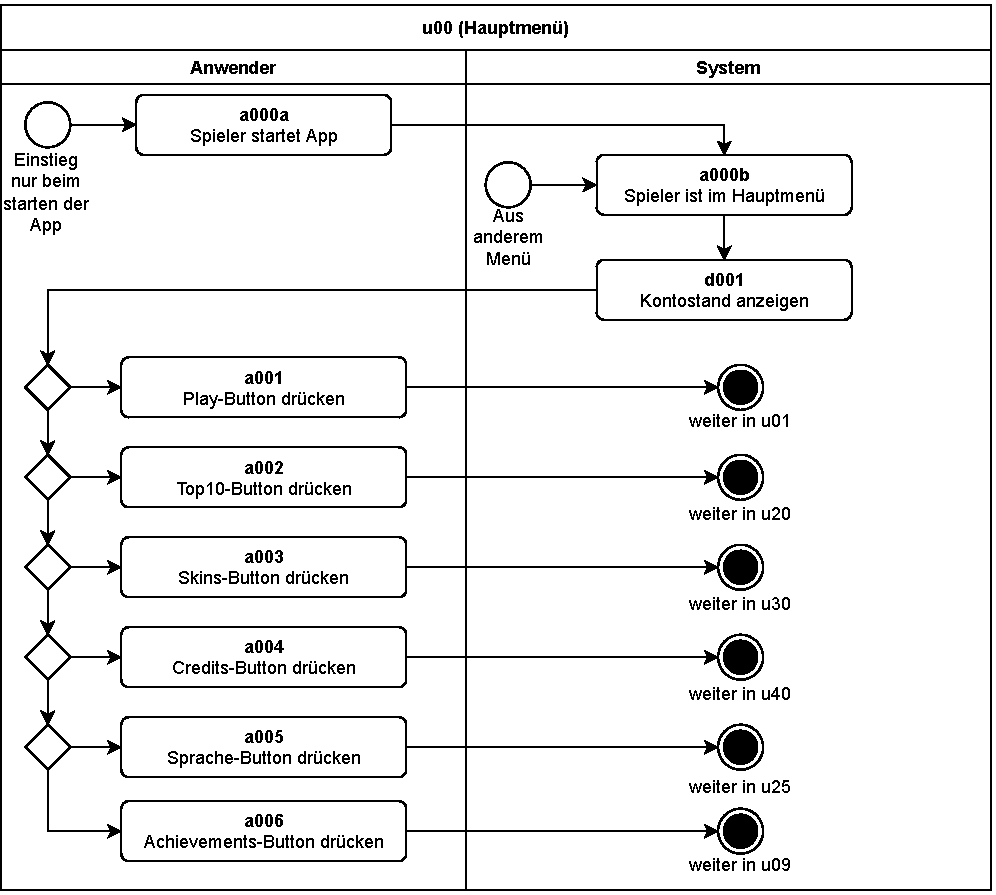
\includegraphics[width=\linewidth]{diagramme/pdf/UML-Activity-u00.pdf}
\captionof{figure}{Aktivität u00 - App-Start / Hauptmenü}\label{fig:dia:mainMenu}
\vspace*{0.5cm}

Figure \ref{fig:dia:mainMenu} stellt den Ablauf der Aktivität u00 dar und in Kapitel \ref{dialog:hauptmenu} wird die dazugehörige Benutzeroberfläche dargestellt. Nach der Installation hat der \gls{spieler} die Möglichkeit, mit einem Klick auf die Anwendung (zu finden in der Liste installierter Apps des Mobilgeräts) das Spiel zu starten. 
Nach maximal fünf Sekunden Ladezeit befindet sich der Spieler dann automatisch im Hauptmenü. Im \hyperref[fig:dia:mainMenu]{Hauptmenü} stehen dem \gls{spieler} fünf verschiedene Buttons zur Verfügung, die ihn zu anderen Screens leiten. Mit dem Play-Button gelangt man zur Spielauswahl. Über den \gls{Top10} Button kann man sich die zehn besten Spiel\-durch\-läufe im \gls{classicMode} und \gls{invasionMode} anschauen.

\vspace{1em}

Im Spiel sind außerdem \glspl{skin} enthalten, die man nach Klicken des Skins-Buttons anschauen und kaufen kann. Mit dem Credits-Button gelangt man zu einem Screen, der ein paar Worte der Entwickler enthält und alle Mitwirkenden am Spiel auflistet. Über den Sprache-Button öffnet sich ein Overlay direkt über dem \hyperref[fig:dia:mainMenu]{Hauptmenü}, dass dem \gls{spieler} die Möglichkeit gibt, die Sprache der gesamten App zu ändern. Die Standard-Sprache ist Englisch. Zuletzt gibt es noch ein weiteres Fenster für Achievements, das über den Achievements-Button aufgerufen werden kann.


\clearpage

\subsubsection{Aktivität u01 - Spielmodus Einstellungen}

\vspace*{1cm}
   
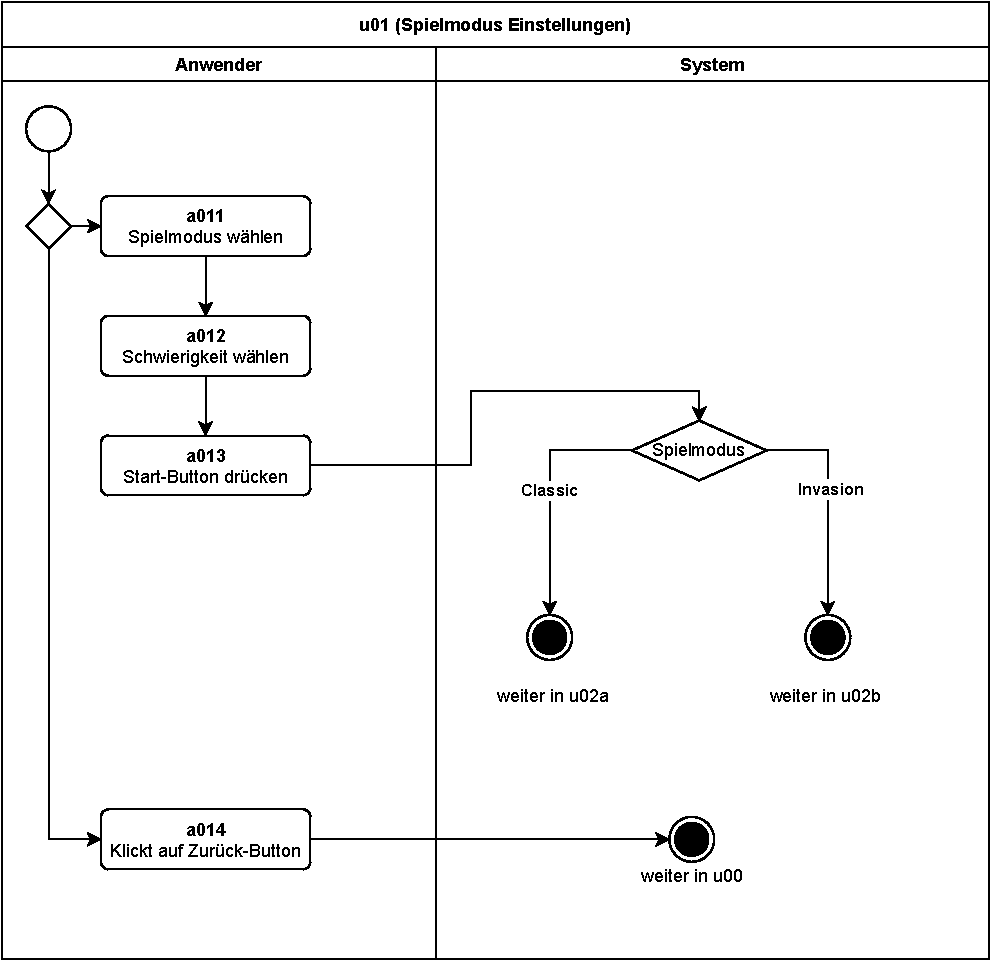
\includegraphics[width=\linewidth]{diagramme/pdf/UML-Activity-u01.pdf}
\captionof{figure}{Aktivität u01 - Spielmodus Einstellungen}\label{fig:dia:gameMode}
\vspace*{0.5cm}

Figure \ref{fig:dia:gameMode} stellt den Ablauf der Aktivität u01 dar und in Kapitel \ref{dialog:einstellungen} wird die dazugehörige Benutzeroberfläche dargestellt.
Hat der \gls{spieler} den Play-Button gedrückt, so gelangt er in ein neues Fenster, dass ihm die Möglichkeit bietet, den Spielmodus (\gls{classicMode}/\gls{invasionMode}) und die Schwierigkeit (Easy, Medium, Hard) einzustellen. Drückt der \gls{spieler} dann den Start-Button, wird eine neue Spielrunde mit den ausgewählten Einstellungen geladen. Über den Zurück-Button gelangt man wieder in das \hyperref[fig:dia:mainMenu]{Hauptmenü} und die Einstellungen werden verworfen.

\clearpage

\subsubsection{Aktivität u02a - Spiel Classic}

\vspace*{1cm}

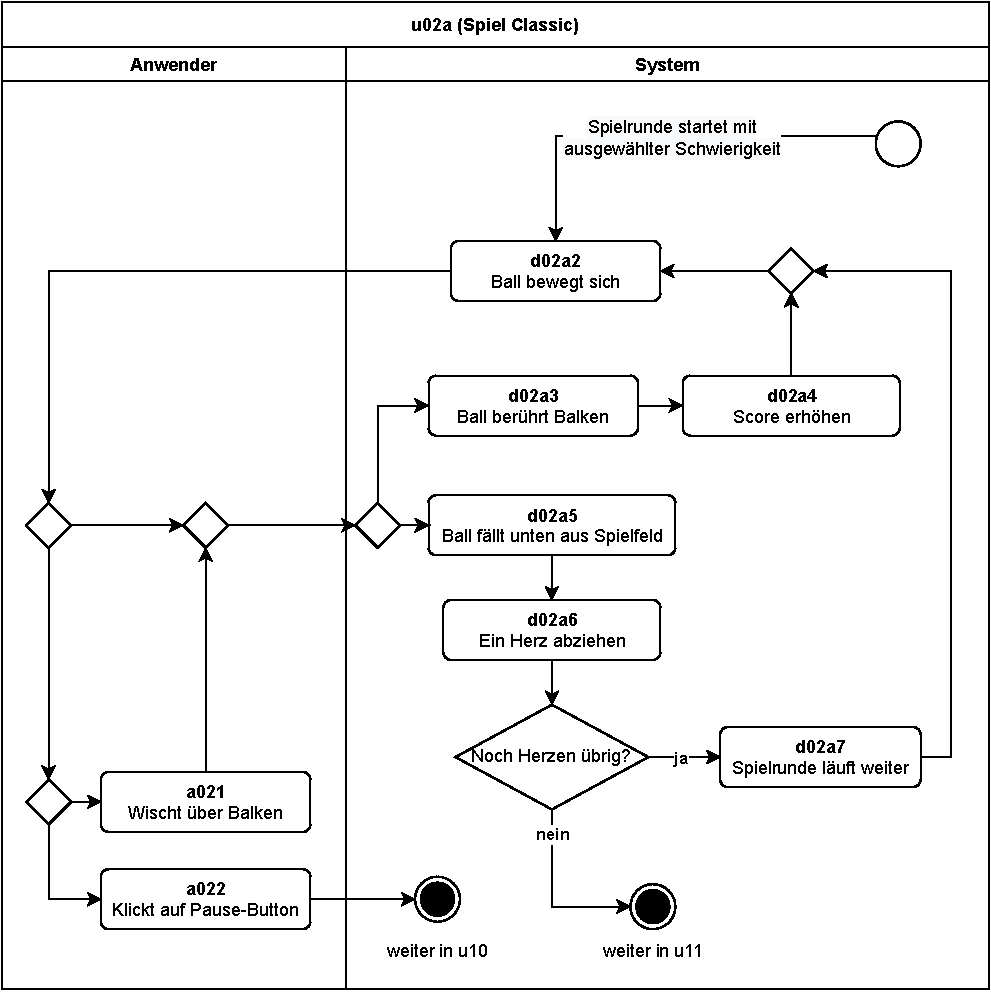
\includegraphics[width=\linewidth]{diagramme/pdf/UML-Activity-u02a.pdf}
\captionof{figure}{Aktivität u02a - Spiel Classic}\label{fig:dia:classic}
\vspace*{0.5cm}

Figure \ref{fig:dia:classic} stellt den Ablauf der Aktivität u02a dar und in Kapitel \ref{dialog:classic} wird die dazugehörige Benutzeroberfläche dargestellt.
Im \gls{classicMode} muss der \gls{spieler} den \gls{ball} mithilfe des \glspl{balken} im \gls{spielfeld} halten, indem er diesen durch Wischen auf dem Screen nach links und rechts bewegt. Beim Starten einer neuen Spielrunde wird diese mit den ausgewählten Einstellungen (Easy/Medium/Hard) initialisiert und der Ball spawnt. Berührt der \gls{ball} den \gls{balken}, die Wände oder Decke des Spielfelds, so prallt er ab und ändert seine Richtung abhängig vom Auftreffwinkel und Auftreffpunkt. Außerdem wird der Score jedes Mal erhöht, wenn der \gls{ball} den \gls{balken} trifft.
Fällt der Ball unten aus dem \gls{spielfeld}, so verliert der Spieler ein Leben (Startet mit 3), der \gls{ball} wird wieder in die Mitte gesetzt und die Runde läuft weiter. Sollte der \gls{spieler} jedoch drei Leben verlieren, so ist die Runde vorläufig zu Ende und der Game-Over Screen wird aufgerufen.
Der Spieler hat jedoch während der gesamten Zeit immer die Möglichkeit zu pausieren und gegebenenfalls die Runde frühzeitig zu beenden.  


\clearpage
\subsubsection{Aktivität u02b - Spiel Invasion}

\vspace*{1cm}

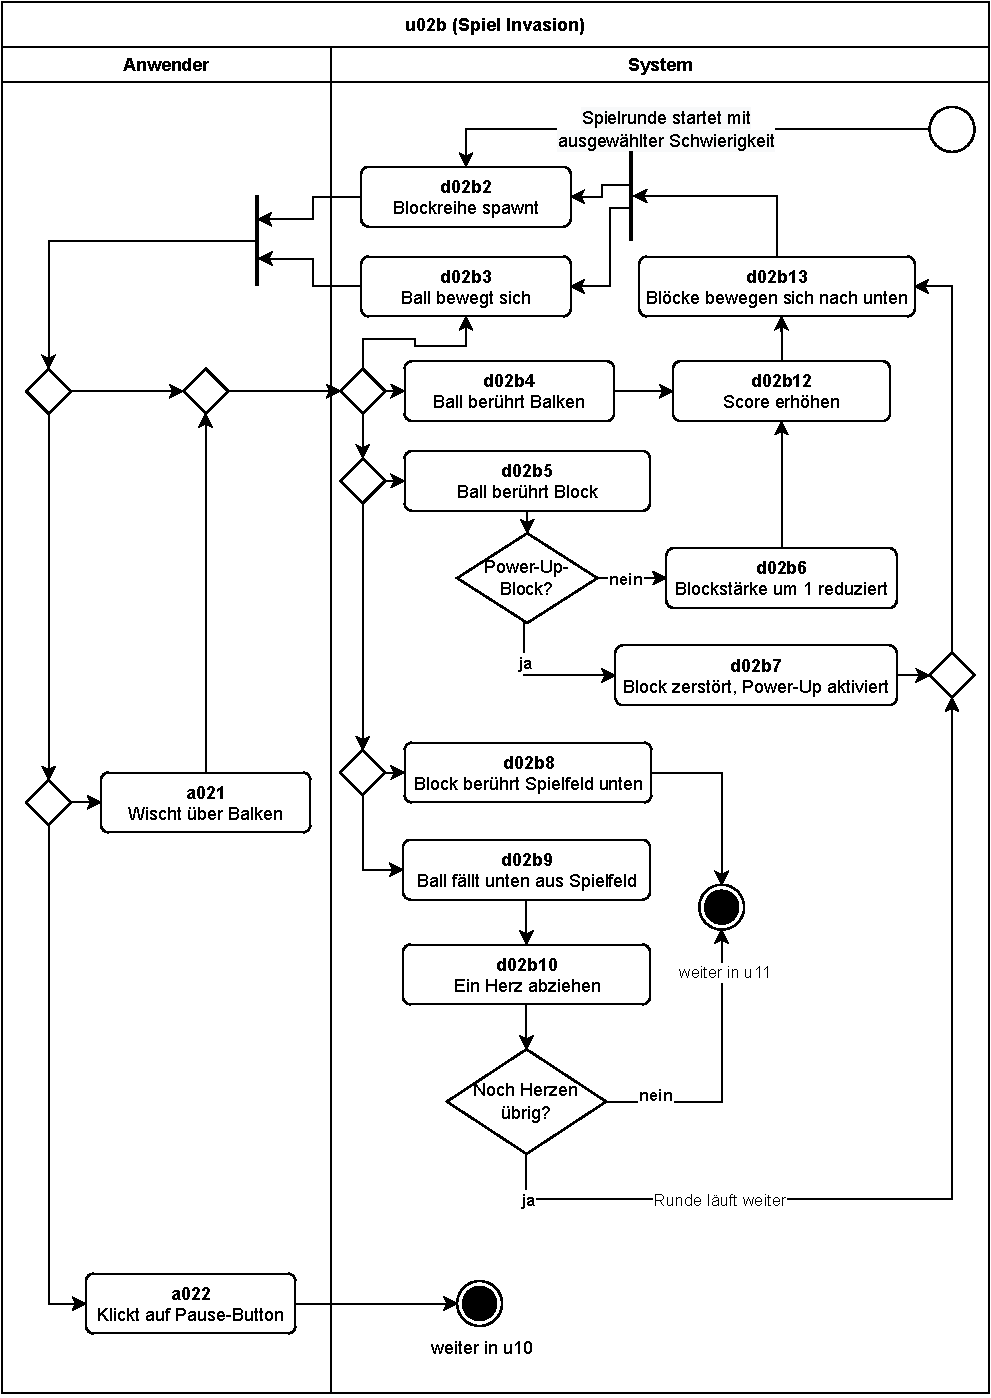
\includegraphics[width=\linewidth]{diagramme/pdf/UML-Activity-u02b.pdf}
\captionof{figure}{Aktivität u02b - Spiel Invasion}\label{fig:dia:invasion}
\vspace*{0.5cm}


\textit{Der Spielmodus Invasion und der damit verbundene Screen sind optional.}
\\
Figure \ref{fig:dia:invasion} stellt den Ablauf der Aktivität u02b dar und in Kapitel \ref{dialog:invasion} wird die dazugehörige Benutzeroberfläche dargestellt.
Der \gls{invasionMode} ist eine Erweiterung zum \gls{classicMode}. Ab Rundenstart spawnt periodisch eine Reihe an Blöcken verschiedener Stärke und vereinzelt mit Power-Ups für den \gls{spieler}. Diese Blöcke müssen mehrmals, je nach der Stärke des Blocks, vom \gls{ball} getroffen werden, um sie zu zerstören. Zerstört der Spieler einen \gls{powerup}-\gls{block}, so erhält der \gls{ball} oder der \gls{spieler} für kurze Zeit eine besondere Eigenschaft (siehe 9.2.1). 
Zusätzlich muss der Spieler darauf achten, dass kein Block den unteren Spielfeldrand berührt. Ansonsten verliert er alle seine Leben und wird direkt zum Game-Over-Menü geleitet. Alle anderen Spielabläufe des \gls{invasionMode} sind identisch zu dem des \gls{classicMode} (5.1.3).


\clearpage

\subsubsection{Aktivität u09 - Sprachauswahl}

\vspace*{1cm}

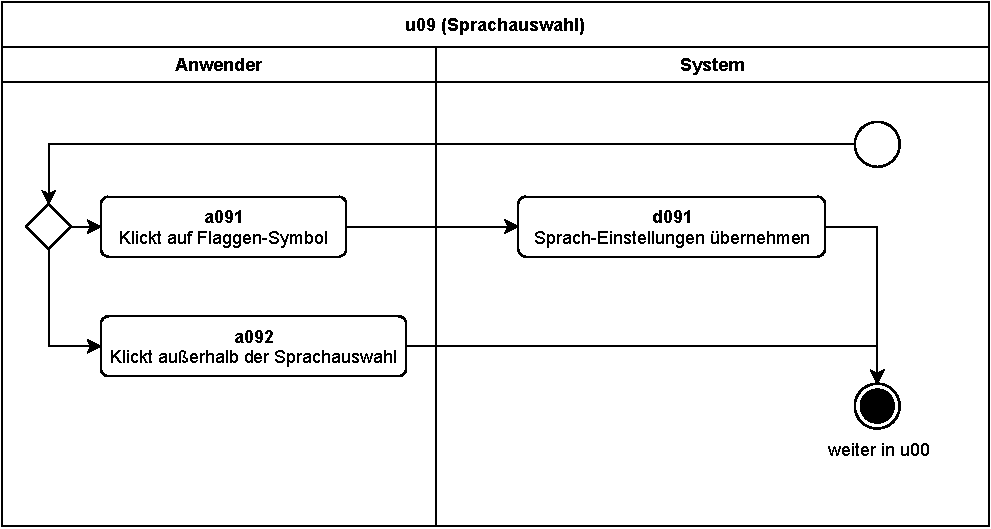
\includegraphics[width=\linewidth]{diagramme/pdf/UML-Activity-u09.pdf}
\captionof{figure}{Aktivität u09 - Sprachauswahl}\label{fig:dia:language}
\vspace*{0.5cm}

\textit{Die Sprachauswahl und das damit verbundene Overlay sind optional.}
\\
Figure \ref{fig:dia:language} stellt den Ablauf der Aktivität u09 dar und in Kapitel \ref{dialog:Sprachauswahl} wird die dazugehörige Benutzeroberfläche dargestellt.
Wurde der Sprache-Button im Hauptmenü gedrückt, öffnet sich ein Overlay. Darin hat der \gls{spieler} die Möglichkeit, die Sprache des Spiels zu ändern, indem er auf eine der verfügbaren Flaggen klickt. Die Standardeinstellung der Sprache ist Englisch. Durch das Klicken außerhalb der Sprachauswahl kommt der \gls{spieler} wieder in das \hyperref[fig:dia:mainMenu]{Hauptmenü} zurück.

\clearpage


\subsubsection{Aktivität u10 - Pause-Menü}


\vspace*{1cm}

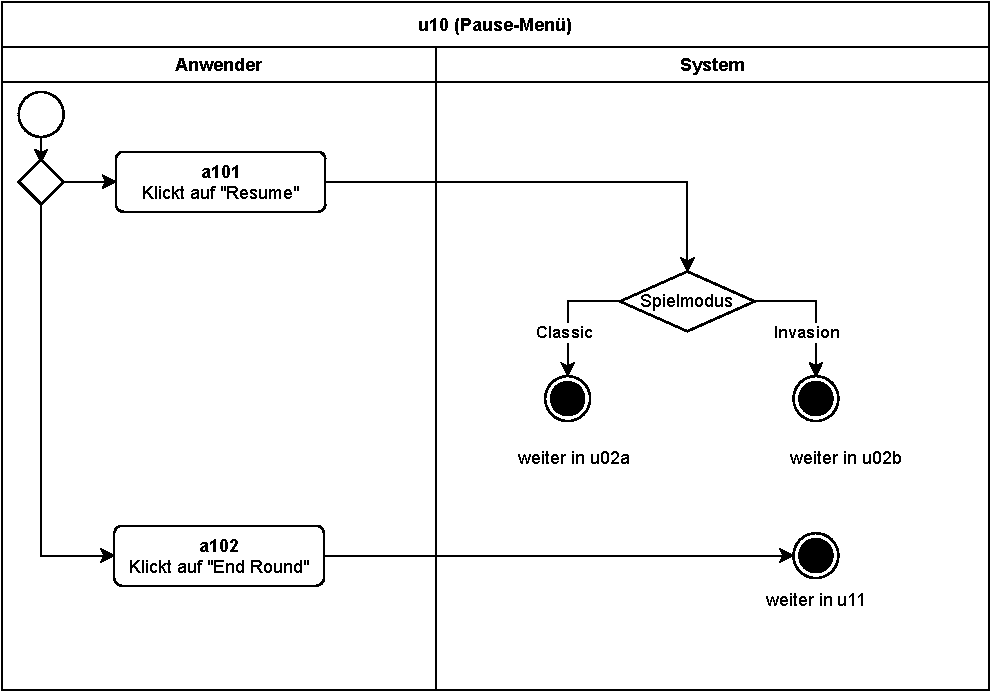
\includegraphics[width=\linewidth]{diagramme/pdf/UML-Activity-u10.pdf}
\captionof{figure}{Aktivität u10 - Pause-Menü}\label{fig:dia:pause}
\vspace*{0.5cm}

Figure \ref{fig:dia:pause} stellt den Ablauf der Aktivität u10 dar und in Kapitel \ref{dialog:pause} wird die dazugehörige Benutzeroberfläche dargestellt.
Während einer aktiven Spielrunde hat der \gls{spieler} die Möglichkeit zu pausieren. Dann wird das Spiel angehalten und ein Overlay öffnet sich. Darin kann der Spieler entweder den Resume-Button klicken, um die jeweilige Runde fortzusetzen, oder auf "End-Round" klicken, um die Runde frühzeitig zu beenden.

\clearpage

\subsubsection{Aktivität u11 - Game-Over-Menü}\label{subsec:u11-gameOver}

\vspace*{1cm}

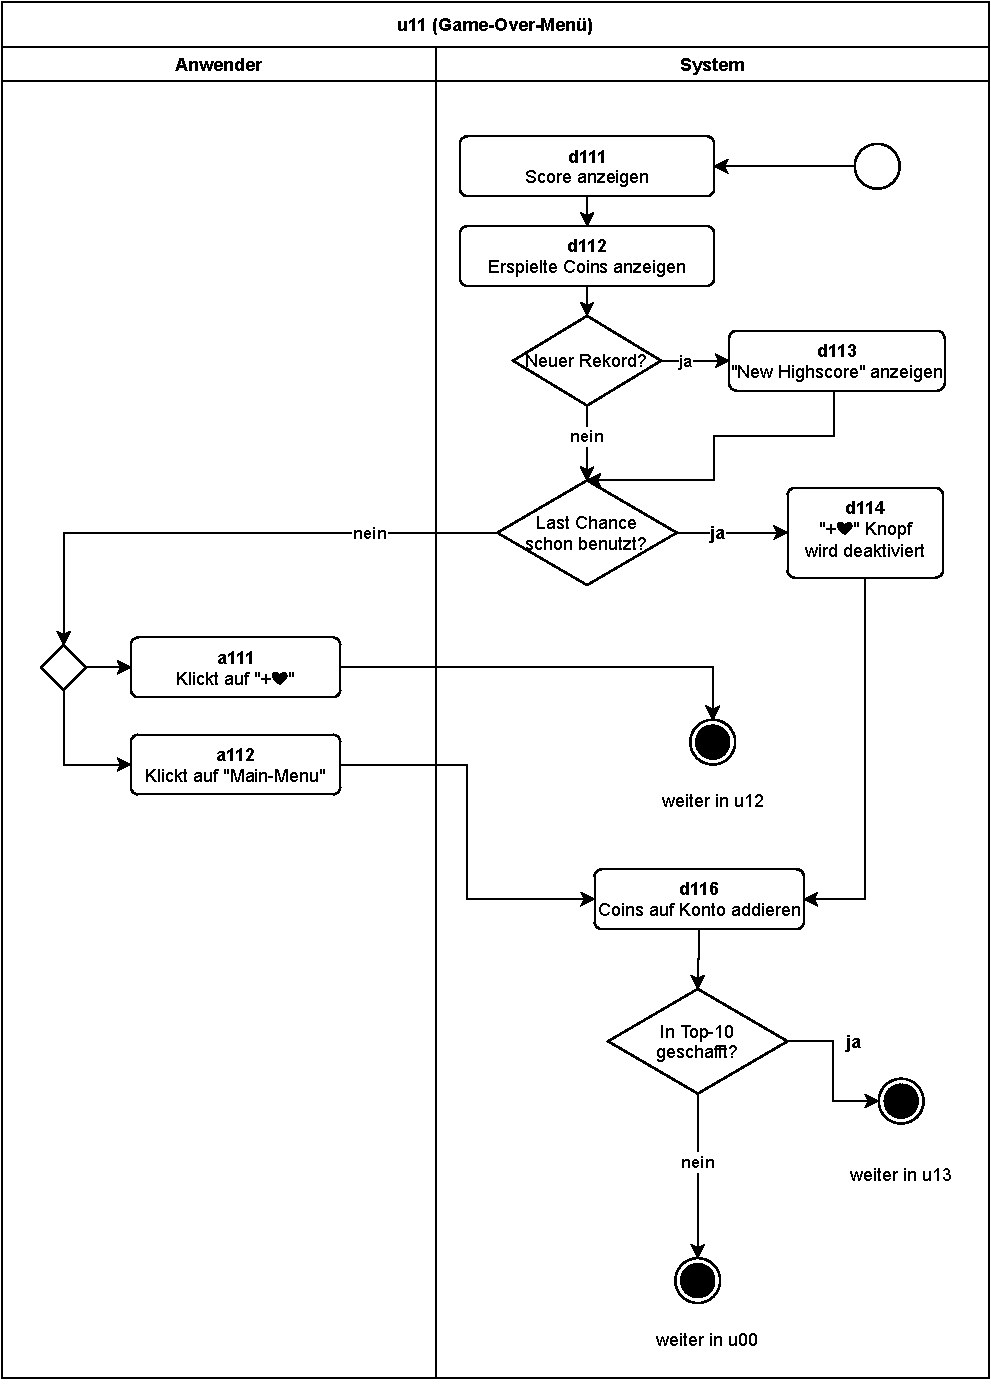
\includegraphics[width=\linewidth]{diagramme/pdf/UML-Activity-u11.pdf}
\captionof{figure}{Aktivität u11 - Game-Over-Menü}\label{fig:dia:gameOver}
\vspace*{0.5cm}

Figure \ref{fig:dia:gameOver} stellt den Ablauf der Aktivität u11 dar und in Kapitel \ref{subsec:u11-gameOverMenu} wird die dazugehörige Benutzeroberfläche dargestellt.
Hat der \gls{spieler} alle seine Leben verloren, oder die Runde im Pause-Menü frühzeitig beendet, so kommt er automatisch in das Game-Over-Menü. Hier werden die erspielten Coins und der bisher erreichte Score angezeigt. Hat er in der Runde einen höheren Score erreicht als einer der Scores in der \gls{Top10} Liste, bekommt der \gls{spieler} die Nachricht „New Highscore“ auf dem Screen angezeigt.

\vspace{1em}

Hat der \gls{spieler} noch keine „Last Chance“ genutzt, so bietet ihm das System einmalig die Möglichkeit, einen Werbeclip zu schauen, um nochmal ein Leben zu erhalten und die Runde fortzusetzen. Verliert der \gls{spieler} auch dieses Leben ist die Runde endgültig zu Ende. Danach werden die erspielten Coins automatisch auf das Spiel-Konto addiert und das System prüft, ob der Score des Spielers hoch genug ist, um in die \gls{Top10} zu kommen. Ist dies der Fall, so wird eine Namenseingabe angezeigt, in der der \gls{spieler} seinen Namen eingeben kann. Hat der \gls{spieler} keine \gls{Top10} Platzierung erreicht, wird das \hyperref[fig:dia:mainMenu]{Hauptmenü} geöffnet.
\clearpage

\subsubsection{Aktivität u12 - Werbung}\label{subsec:u12-ads}

\vspace*{1cm}

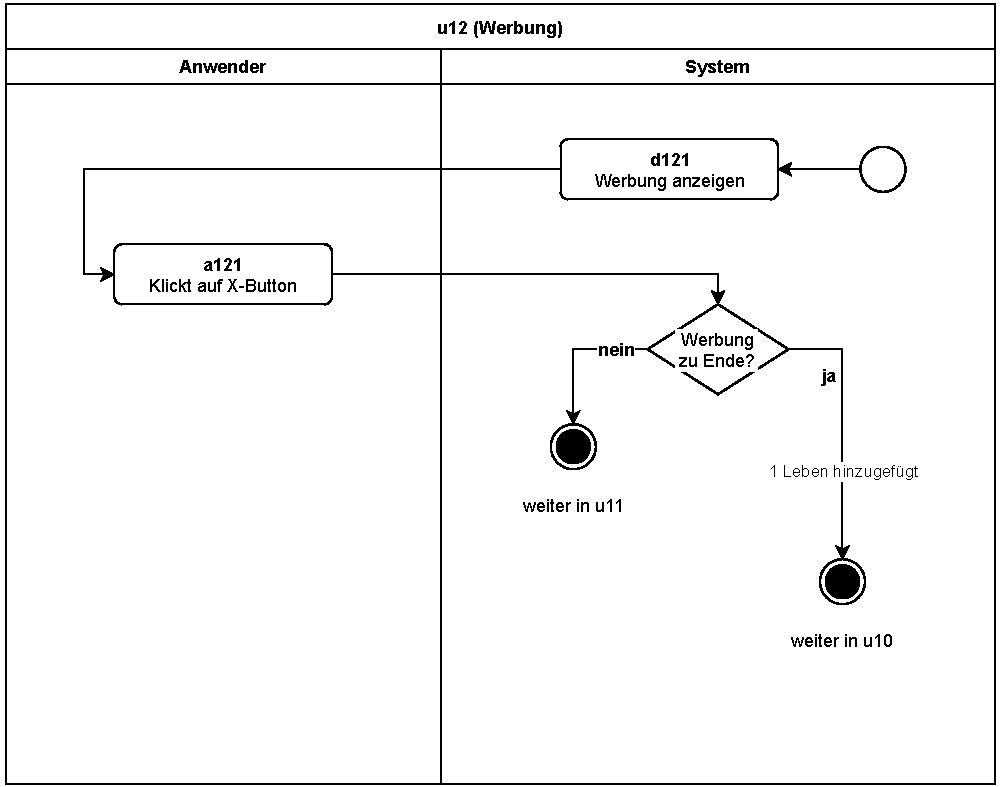
\includegraphics[width=\linewidth]{diagramme/pdf/UML-Activity-u12.pdf}
\captionof{figure}{Aktivität u12 - Werbung}\label{fig:dia:ads}
\vspace*{0.5cm}

Figure \ref{fig:dia:ads} stellt den Ablauf der Aktivität u12 dar und in Kapitel \ref{dialog:Werbung} wird die dazugehörige Benutzeroberfläche dargestellt.
Entscheidet sich der \gls{spieler} Werbung anzuschauen, so hat er die Möglichkeit, diese über den X-Button wieder zu schließen. Ist die Werbung zu diesem Zeitpunkt noch nicht vollständig durchgelaufen, so wird der \gls{spieler} wieder in das Game-Over-Menü weitergeleitet. Hat er sich die Werbung jedoch vollständig angeschaut, so erhält er ein extra Leben und wird zum Pause-Menü weitergeleitet, sodass die Runde fortgesetzt werden kann. Bei Game-Over durch die Berührung eines Blocks mit dem unteren Spielfeldrand, wird die Spielrunde nach dem schauen der Werbung neu initialisiert.

\clearpage

\subsubsection{Aktivität u13 - Namenseingabe}

\vspace*{1cm}

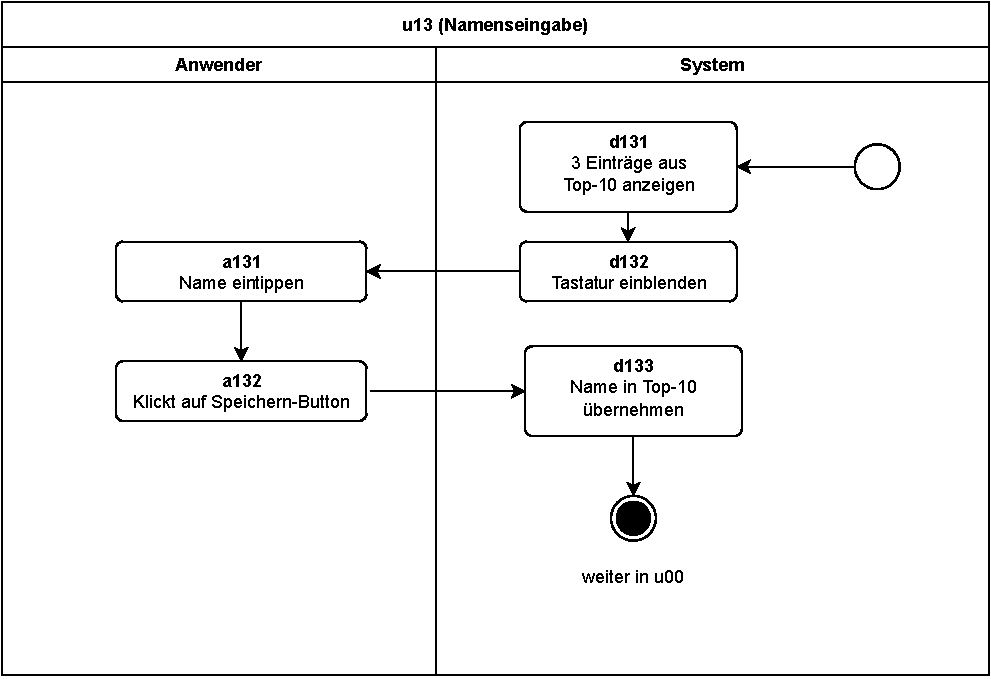
\includegraphics[width=\linewidth]{diagramme/pdf/UML-Activity-u13.pdf}
\captionof{figure}{Aktivität u13 - Namenseingabe}\label{fig:dia:highscore}
\vspace*{0.5cm}

Figure \ref{fig:dia:highscore} stellt den Ablauf der Aktivität u13 dar und in Kapitel \ref{dialog:Namenseingabe} wird die dazugehörige Benutzeroberfläche dargestellt.
Hat der \gls{spieler} nach der Runde eine \gls{Top10} Platzierung erreicht, so wird die Namenseingabe angeboten. Es wird, sofern vorhanden, ein Eintrag der Platzierungen genau vor und einer genau hinter dem des erreichten Scores angezeigt. Unterhalb dieser Anzeige wird die Tastatur
eingeblendet und der \gls{spieler} hat so die Möglichkeit seinen Namen einzutippen und anschließend durch den Klick auf den Speichern-Button seinen Namen in Zusammenhang mit dem Schwierigkeitsgrad und erreichten Score in den \gls{Top10} zu sichern. Danach wird der \gls{spieler} wieder in das \hyperref[fig:dia:mainMenu]{Hauptmenü} geleitet.

\clearpage

\subsubsection{Aktivität u20 - Top-10 Liste}

\vspace*{1cm}

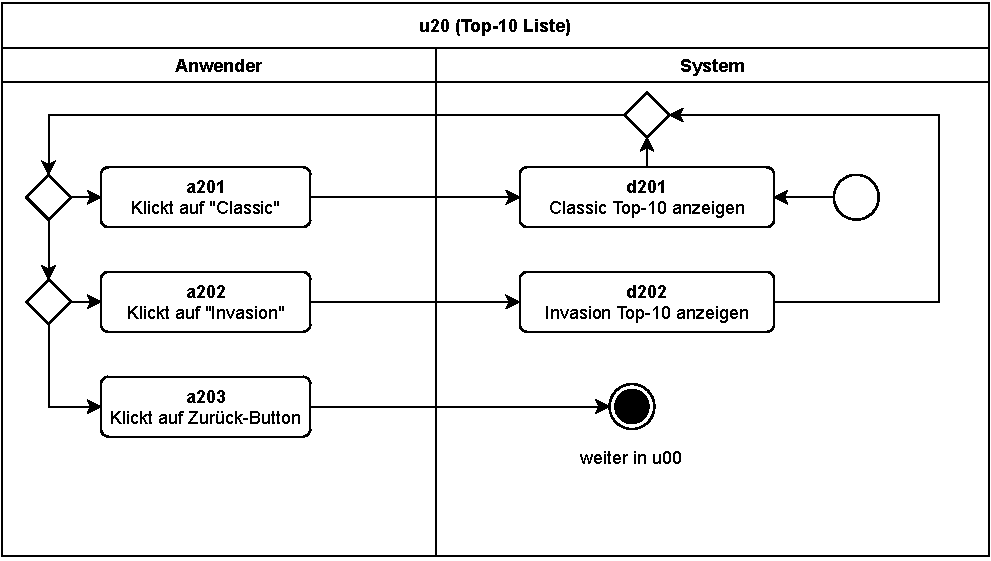
\includegraphics[width=\linewidth]{diagramme/pdf/UML-Activity-u20.pdf}
\captionof{figure}{Aktivität u20 - Top-10 Liste}\label{fig:dia:top10}
\vspace*{0.5cm}

Figure \ref{fig:dia:top10} stellt den Ablauf der Aktivität u20 dar und in Kapitel \ref{dialog:top10} wird die dazugehörige Benutzeroberfläche dargestellt.
Klickt der \gls{spieler} im \hyperref[fig:dia:mainMenu]{Hauptmenü} auf den \gls{Top10}-Button, so werden ihm standardmäßig die 10 höchsten Scores im \gls{classicMode} in Listenform angezeigt. Durch einen Klick auf den Invasion-Button ändert sich die Liste und zeigt dann die 10 höchsten Scores im \gls{invasionMode} an. Analog dazu führt der Classic-Button zur Top-10 Liste des \gls{classicMode} zurück.
Über den Zurück-Button gelangt der \gls{spieler} wieder in das \hyperref[fig:dia:mainMenu]{Hauptmenü}.

\clearpage

\subsubsection{Aktivität u25 - Achievements}

\vspace*{1cm}

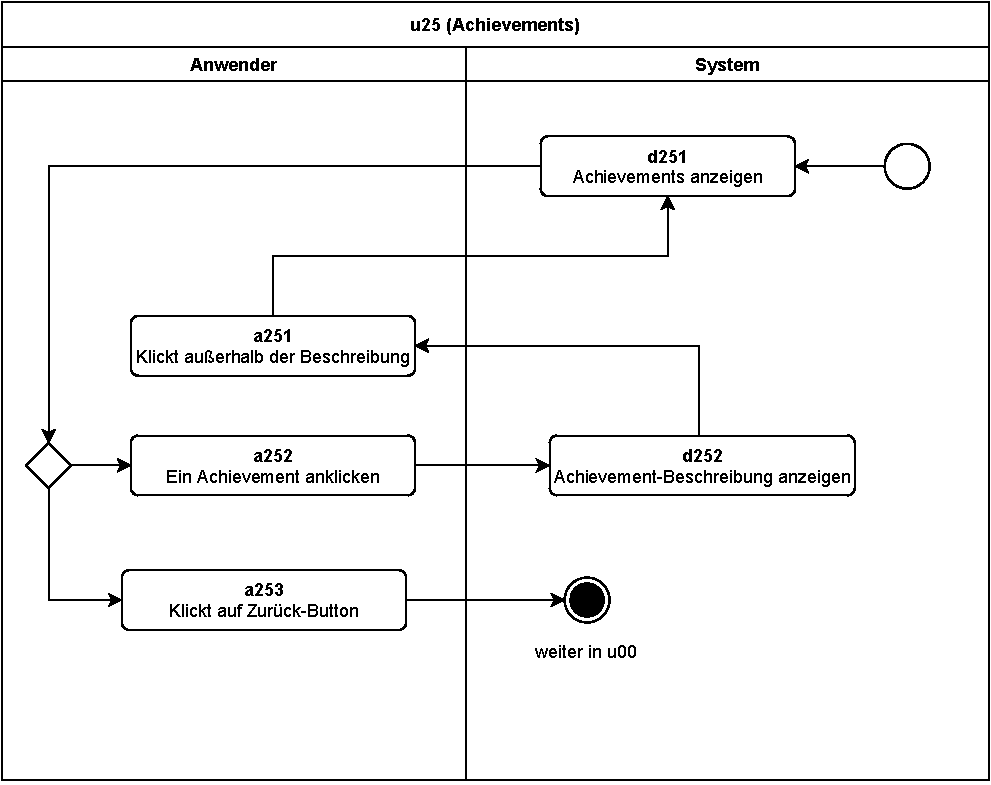
\includegraphics[width=\linewidth]{diagramme/pdf/UML-Activity-u25.pdf}
\captionof{figure}{Aktivität u25 - Achievements}\label{fig:dia:achievements}
\vspace*{0.5cm}

\textit{Die Achievements und der damit verbundene Screen sind optional.}
\\
Figure \ref{fig:dia:achievements} stellt den Ablauf der Aktivität u25 dar und in Kapitel \ref{dialog:Achievements} wird die dazugehörige Benutzeroberfläche dargestellt.
Über den Achievements-Button gelangt der \gls{spieler} auf einen Screen, der alle seine bisher erreichten Achievements anzeigt. Noch nicht erreichte Achievements sind ausgegraut. Wird auf eines der Symbole geklickt, so öffnet sich ein Overlay und der Spieler kann die Beschreibung des jeweiligen Achievements nachlesen. Klickt der Spieler außerhalb des Overlays, kommt er zurück auf die Ansicht aller Achievements. Durch das Klicken des Zurück-Buttons gelangt der Spieler dann wieder in das \hyperref[fig:dia:mainMenu]{Hauptmenü}. 

\clearpage

\subsubsection{Aktivität u30 - Skin-Auswahl}

\vspace*{1cm}

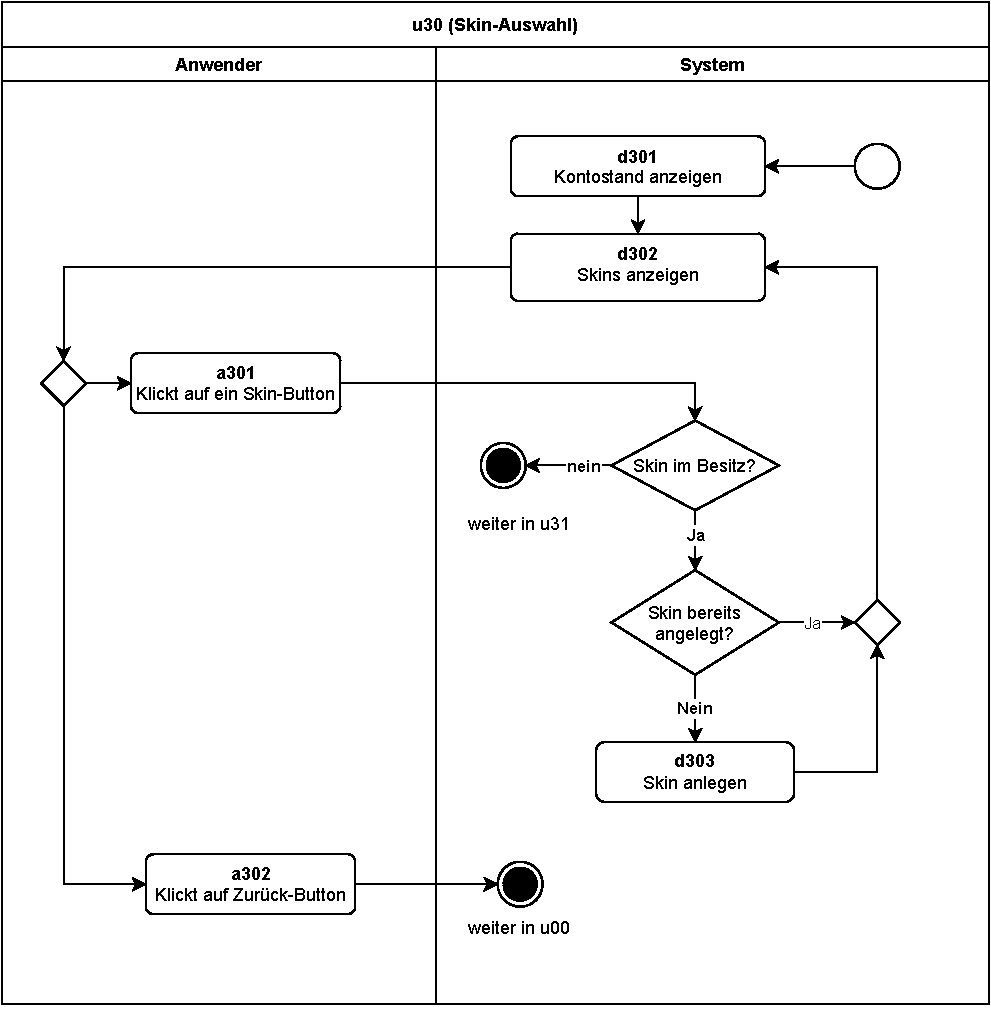
\includegraphics[width=\linewidth]{diagramme/pdf/UML-Activity-u30.pdf}
\captionof{figure}{Aktivität u30 - Skin-Auswahl}\label{fig:dia:skins}
\vspace*{0.5cm}

Figure \ref{fig:dia:skins} stellt den Ablauf der Aktivität u30 dar und in Kapitel \ref{dialog:skins} wird die dazugehörige Benutzeroberfläche dargestellt.
Klickt der Spieler auf den Skins-Button, so gelangt er auf einen Screen, der ihm alle im Spiel verfügbaren \glspl{skin} des \glspl{ball}, des \glspl{tail}, des Balkens und des Hintergrunds anzeigt. Zusätzlich sieht er hier auch seinen aktuellen Kontostand. Durch Klicken eines Skin-Buttons wird ein Overlay geöffnet, das dem \gls{spieler} die Möglichkeit bietet, den \gls{skin} zu kaufen oder anzulegen. Ist der ausgewählte \gls{skin} bereits angelegt, so wird das Overlay nicht geöffnet und der Spieler bleibt auf der Anzeige aller \glspl{skin}.
\clearpage

\subsubsection{Aktivität u31 - Skin-Kauf}

\vspace*{1cm}

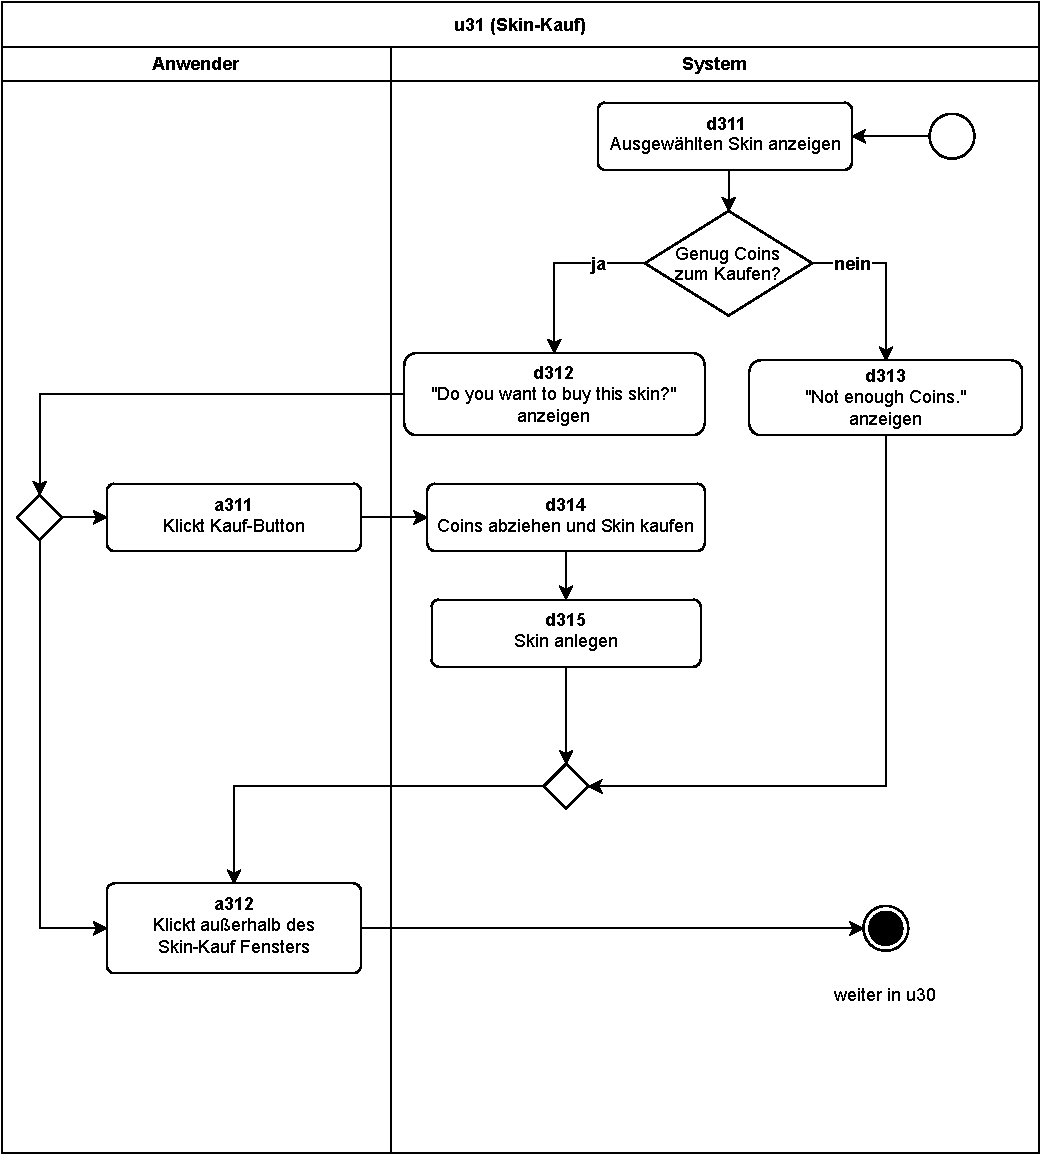
\includegraphics[width=\linewidth]{diagramme/pdf/UML-Activity-u31.pdf}
\captionof{figure}{Aktivität u31 - Skin-Kauf}\label{fig:dia:skinPurchase}
\vspace*{0.5cm}

Figure \ref{fig:dia:skinPurchase} stellt den Ablauf der Aktivität u31 dar und in Kapitel \ref{dialog:skinkauf} wird die dazugehörige Benutzeroberfläche dargestellt.
Hat der \gls{spieler} einen \gls{skin} ausgewählt, so wird ein Overlay geöffnet. Ist der \gls{skin} noch nicht in seinem Besitz, so wird vom System geprüft, ob genügend Coins für den Kauf des \glspl{skin} vorhanden sind. Ist dies der Fall, so wird die Nachricht „Do you want to buy this skin?“ angezeigt. Entscheidet sich dann der \gls{spieler} diesen zu kaufen, so werden die benötigten Coins von seinem Konto abgezogen, der \gls{skin} freigeschaltet und direkt angelegt. 
Fehlen dem \gls{spieler} noch Coins für den \gls{skin}, so zeigt das System die Nachricht „Not enough Coins“ an. Mit einem Klick außerhalb des Overlays kommt der \gls{spieler} dann wieder zurück auf die Anzeige aller \glspl{skin}.

\clearpage

\subsubsection{Aktivität u40 - Credits}

\vspace*{1cm}

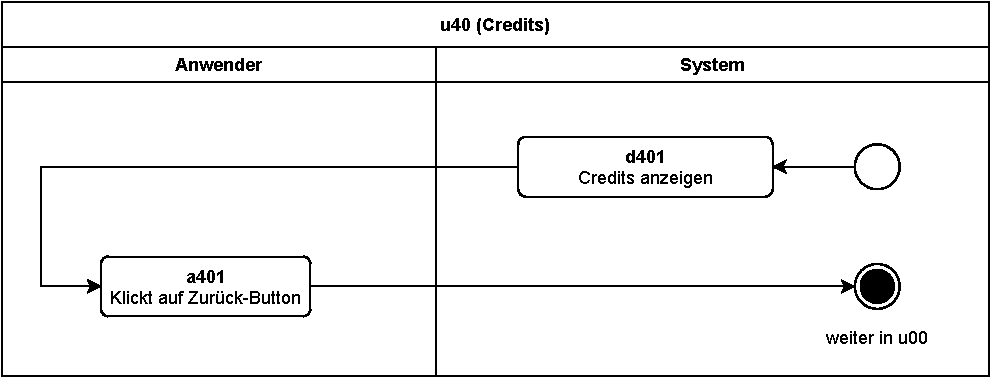
\includegraphics[width=\linewidth]{diagramme/pdf/UML-Activity-u40.pdf}
\captionof{figure}{Aktivität u40 - Credits}\label{fig:dia:credits}
\vspace*{0.5cm}

Figure \ref{fig:dia:credits} stellt den Ablauf der Aktivität u40 dar und in Kapitel \ref{dialog:credits} wird die dazugehörige Benutzeroberfläche dargestellt.
Bei einem Klick auf den Credits-Button muss das System dem \gls{spieler} die Credits anzeigen. 
Dieser enthält paar Worte der Entwickler und listet alle Mitwirkenden am Spiel auf. 
Der \gls{spieler} hat die Möglichkeit, den Credits-Screen durch einen Klick auf den Zurück-Button zu verlassen und das \hyperref[fig:dia:mainMenu]{Hauptmenü} zu erreichen.

\clearpage
